\documentclass[manuscript,review,anonymous]{acmart}

%%% Packages %%%
\usepackage{booktabs}
\usepackage{multirow}
\usepackage{graphicx}
\usepackage{subcaption}
\usepackage{xcolor}
\usepackage{tikz}
\usetikzlibrary{arrows.meta}
\graphicspath{{figures/}}

\renewcommand{\sectionautorefname}{Section}
\renewcommand{\subsectionautorefname}{Section}
\renewcommand{\subsubsectionautorefname}{Section}

%%% ACM Metadata %%%
\acmConference[CHI '27]{ACM CHI Conference on Human Factors in Computing Systems}{April 26--May 1, 2027}{Yokohama, Japan}
\acmYear{2027}
\acmISBN{}
\acmDOI{}
\acmPrice{}

\setcopyright{none}

\title{Admitting AI Agents: Agentic Readiness and Adoption in an Automation Marketplace}

\begin{document}

\begin{abstract}
Automation tool marketplaces are increasingly opened to machine consumers---AI
agents that autonomously discover, invoke, and pay for tools. On the Apify
Store, this opening is architectural: a tool is \emph{agentic-ready}---eligible
for agent-initiated use---only if it runs with limited permissions and no
standby mode. We study how agentic readiness shapes marketplace outcomes, using
a census of 67{,}609 tools from 5{,}789 developers (57{,}032 pay-per-event
tools, 53{,}502 with architecture data) and within-developer fixed-effects
models. Within the same developer---among the 343 who publish both tool
types---agentic-ready tools attract a large positive mean adoption gap
($p < 10^{-10}$): 40\% to 72\% on the
$\log(1+\text{monthly\_users})$ scale depending on weighting (72\% under our
preferred equal-developer-weighted estimator), and several-fold larger on the
raw monthly-user count scale; a within-developer similarity match attenuates
the gap to roughly 29\%, so the premium is partly a tool-type composition
effect, but a positive mean premium persists. The association operates on both
the extensive margin (a
17-percentage-point higher probability of having any users) and the intensive
margin (60\% more on the log-plus-one scale conditional on traction). The
association is positive across most tool categories (Bonferroni-significant in 7 of 15
under primary-category assignment, 12 of 18 under multi-hot), and the
association survives excluding whale developers and is directionally
triangulated by propensity-score weighting. In contrast, despite their higher
adoption, we find no robust evidence of higher within-group concentration: Gini
coefficients are nearly identical across the two sets (0.935 versus 0.946), and
upper-tail differences are too imprecisely estimated to be informative. Because
we observe readiness rather than agent use, the association may reflect agent
routing, developer self-selection, the architecture's intrinsic appeal, or some
combination. These findings surface a design-relevant empirical signal: the
admission boundary doubles as a discovery and governance boundary---the same
limited-permissions, non-standby requirements that gate agent access also
decide which tools machine consumers can find at all---and a single metric like
\texttt{monthly\_users} can no longer separate human- from agent-driven
adoption.
\end{abstract}

\keywords{automation marketplace, agentic economy, platform governance, marketplace concentration, adoption gap}

\maketitle

% !TEX root = ../main.tex
\section{Introduction}
\label{sec:introduction}

Automation tool marketplaces---platforms where developers publish reusable
scripts, scrapers, and integrations---are being opened to a new kind of
consumer: AI agents that autonomously discover, invoke, and pay for tools, a
shift documented in census analyses of the MCP tool ecosystem
\cite{stein2026mcpecosystem} and the GPT Store \cite{su2024gptstore}. For a tool
to enter an agent's
reach, however, it must first satisfy a platform-imposed architecture. On the
Apify Store, a tool is \emph{agentic-ready} only if it runs with limited
permissions and no standby mode. Agentic readiness is thus not a label a
developer claims, but a set of architectural constraints the platform enforces
on which tools machine consumers may touch. Yet little is known about how this
readiness architecture shapes adoption and concentration across the
marketplace.

Automation tool marketplaces are a distinct platform
type with four structural features: they host \emph{single-function} tools
rather than the multi-feature applications that mobile app stores manage
through update review \cite{comino2019appstore}, use
predominantly \emph{usage-based}
pricing rather than subscription or purchase models, organize tools through
\emph{category taxonomies} for both human and programmatic discovery, and rely
on open developer-side participation that produces a long-tailed distribution
of activity. They are not app stores (tools are headless scripts, not
interactive applications), not API marketplaces (tools encapsulate orchestrated
workflows rather than exposing raw endpoints), and not integration platforms
(tools are standalone rather than connectors between services). We describe
these features concretely for Apify in \autoref{sec:context}.\label{sec:bg:automation}

We analyze the \emph{Apify Store}, a public automation marketplace hosting
67,609 tools (``actors'') built by 5,789 developers. We define a pay-per-event
(PPE) tool as \emph{agentic-ready} when it is configured with limited
permissions and no standby mode---two architectural properties that, in the
platform's design, determine whether a tool can be autonomously discovered and
invoked by agents. 50{,}917 of the 53{,}502 PPE tools with architecture data
(95\%) satisfy this definition. We study how agentic readiness is associated
with adoption and concentration, using within-developer fixed effects that
compare agentic-ready and non-agentic-ready tools published by the \emph{same}
developer.

Prior work leaves four gaps: no empirical study of automation tool marketplaces
as a distinct platform type, no quantification of the adoption gap associated
with agentic readiness, no documentation of category-level heterogeneity in
that gap, and no analysis of whether agentic readiness is associated with
marketplace concentration. Our study addresses all four.

This study's organizing question is: what adoption and concentration
differences are associated with a platform's readiness boundary---the
constraints it imposes on which tools machine consumers may use? We find three
things.

First, agentic readiness is strongly associated with adoption. Within the same
developer---specifically the 343 who publish both agentic-ready and
non-agentic-ready tools---agentic-ready tools attract a large positive mean
adoption gap ($p < 10^{-10}$): 40\% to 72\% on the
$\log(1+\text{monthly\_users})$ scale depending on weighting, and several-fold
larger on the count scale; a within-developer similarity match confirms a positive mean premium of roughly 29\%,
indicating that tool-type composition explains part of the raw gap but not all of it. Second, the association also appears on both the
extensive and conditional intensive margins: agentic-ready tools are 17
percentage points more likely to have any users at all, and, conditional on
having users, they attract 60\% more on the log-plus-one scale. Third, the
association is positive across
categories---Bonferroni-significant in 7 of 15 under primary-category assignment
and 12 of 18 under multi-hot, in tool-level regressions---but we find no robust
evidence of higher concentration: Gini coefficients are nearly identical across
agentic-ready and non-agentic-ready tools (0.935 versus 0.946), and upper-tail
differences are too imprecisely estimated to be informative.

Across these findings, the through-line is the readiness boundary: tools a
platform configures for agent-initiated use attract substantially more
adoption, without any detectable increase in concentration. This adoption
premium is large and
consistent. The observed premium attaches to platform readiness; distinguishing agent routing from correlated architectural choices requires agent-side traffic data.

To understand how agentic readiness shapes marketplace stratification, we
organize the analysis around three research questions:

\begin{description}
  \item[RQ1.] What is the adjusted association between agentic readiness and
    tool adoption, after controlling for developer heterogeneity and tool
    characteristics?
  \item[RQ2.] On which margin of adoption does the association operate---the
    extensive margin (any users) or the intensive margin (users conditional on
    traction)---and which candidate mechanisms the data can and cannot rule
    out?
  \item[RQ3.] How does the association vary across tool categories, and is
    agentic readiness associated with higher or lower within-group adoption
    inequality?
\end{description}

This study makes two contributions to HCI and platform studies:

\begin{enumerate}
  \item \textbf{Quantifying the adoption premium of agentic readiness.} Within
    the same developer, agentic-ready tools attract a large, consistently
    positive adoption gap (40\% to 72\% on the log-plus-one scale) across both
    the extensive and intensive margins, with no robust evidence of a
    corresponding increase in within-group concentration.

  \item \textbf{The admission boundary as a governance boundary.} This premium
    reveals a design-relevant empirical signal: an automation marketplace's
    permission architecture---the limited-permissions, non-standby criteria that
    gate agent access---doubles as its discovery architecture, so access rules
    allocate visibility across human users, agent users, and developers.
\end{enumerate}

We next describe the setting, data and methods, results, and their
implications for dual-audience governance.

% !TEX root = ../main.tex
\section{Related Work}
\label{sec:background}

This section situates our study within two bodies of prior work: empirical
studies of software marketplaces and platform governance, and research on
interaction modality and dual-audience design.

%% ─────────────────────────────────────────────
\subsection{Software Marketplaces and Platform Governance}
\label{sec:rw:marketplace}

A substantial body of work examines software marketplaces, primarily mobile app
stores: sales rank strongly shapes mobile-app demand
\cite{ghose2014apppricing}, platform-owner entry into complementor markets
induces complementor responses
\cite{wen2019platformowner}, and app updates and category positioning predict
adoption better than review scores \cite{janssen2022googleplay}, while update
management is a strategic lever that differs across app stores
\cite{comino2019appstore}. More recently,
\citet{su2024gptstore} documents the OpenAI GPT Store's extreme concentration
and ``supply without demand,'' and \citet{stein2026mcpecosystem} documents the
MCP ecosystem's reshaping of developer effort. Platform governance research
\cite{rietveld2021platform} explains how such outcomes arise: certification can
amplify concentration by disproportionately benefiting already-popular apps
\cite{rietveld2021marketorchestrators};
boundary resources mediate the owner--complementor relationship
\cite{eaton2015governance,tiwana2015platformecosystems}; and two-sided market
theory \cite{rochet2003twosided} and network effects \cite{caillaud2003chicken}
explain winner-take-all dynamics, with \citet{boudreau2012complementors} showing
that more complementors can reduce individual incentives even as aggregate
value rises. Concentration is standardly measured with Gini coefficients and
HHI, as in analyses of the GPT Store \cite{su2024gptstore}, and the
``superstar'' phenomenon is well-documented
\cite{aguiar2018platforms}. These studies establish heavy-tailed adoption and
platform design effects, but none examines automation marketplaces, or whether
design decisions that introduce new consumption modalities (such as agentic
access) are associated with redistributed concentration.

%% ─────────────────────────────────────────────
\subsection{Agents as Users and Dual-Audience Design}
\label{sec:rw:agentic}

The term ``agentic economy'' describes the emerging ecosystem in which AI
agents act as autonomous consumers of digital services---discovering tools,
negotiating access, executing tasks, and making payments without continuous
human oversight. Governing such agentic systems is an emerging policy concern
\cite{shavit2023practices}. This shift is enabled by large
language models (LLMs) with tool-use capabilities
\cite{schick2023toolformer,qin2024toolllm}, standardized tool-calling protocols
such as MCP---now spanning a large tool ecosystem
\cite{stein2026mcpecosystem}---and JSON-schema-based function calling
\cite{openai2024function}, and payment infrastructure that permits
machine-initiated transactions.

For automation marketplaces, the agentic transition is a change in
\emph{interaction modality}: where a human once browsed a catalog, filled a
form, and clicked run, an agent now discovers via semantic search, generates
parameters from a schema, and pays through pre-authorized billing. These
changes may favor tools that are well-documented and schema-rich.

We treat this modality transition as the paper's theoretical object of study,
rather than as background context, and ground it in four intersecting HCI
lineages.

\emph{Human--AI interaction.} Work on human--AI collaboration establishes
guidelines for systems that collaborate with users \cite{amershi2019guidelines}
and examines how humans and agents negotiate roles beyond a linear
``user specifies, agent executes'' model \cite{zhou2024nonlinear}. Our setting
asks what changes when the ``user'' is itself an agent.

\emph{Agents as users, and machine legibility.} A growing literature treats AI
agents as end-users with their own needs: interface design alone drives large
performance gains for agents \cite{yang2024sweagent}. API usability research
establishes that interfaces demand explicit design for their users
\cite{myers2016api}; extending this principle to machine consumers suggests
that interfaces built for one audience can become illegible to another. These
motivate our question of whether a \emph{payment-eligibility signal} is
associated with measurable adoption differences.

\emph{Developer experience and mediated work.} Developer experience (DevEx) work
\cite{fagerholm2012developer,weisz2025codeassistant} and algorithmic-mediation
research \cite{eslami2015algorithmic,lee2015working} show that platforms
designed for one population can be illegible to another, and recommendation
systems have been framed as requiring fairness across multiple stakeholder
groups \cite{burke2017multisided}---direct concerns for a marketplace whose
audience is now heterogeneous.

\emph{Hybrid intelligence and automation paradigms.} Hybrid-intelligence
research frames human--AI collaboration as a division of labor
\cite{dellermann2019hybrid}, and automation-paradigm studies show that
``do it for me'' versus ``do it with me'' is a design decision with distinct
consequences for control and trust \cite{khurana2025doitforme}. Our paper asks
what a design decision optimizing for one modality does to the other.

Apify's agentic-readiness boundary is a concrete instance of such a design
decision: it admits tools with limited permissions and no standby mode to
agent-initiated use. Whether this readiness is associated with measurable
adoption differences is the empirical question this paper studies.

% !TEX root = ../main.tex
\section{Research Context: The Apify Store}
\label{sec:context}

This section describes the institutional setting, pricing architecture, and the
platform's access boundary that structure our analysis.

%% ─────────────────────────────────────────────
\subsection{Platform Overview}

Apify is a cloud automation platform providing serverless infrastructure for
web scrapers, browser automations, and data-extraction workflows. Developers
build discrete tools called \emph{actors}---self-contained programs that accept
structured input, execute a task, and return structured output---and publish
them to the \emph{Apify Store}, a public marketplace where end users discover,
configure, and run tools. The Store is a two-sided market: developers supply
actors and earn revenue from usage, while users pay on a usage or rental basis
(or use free actors) to access a growing catalog of pre-built automations.

%% ─────────────────────────────────────────────
\subsection{Pricing Architecture}

The Store supports three pricing models. \emph{Pay-per-event} (PPE) is the
dominant model (84\% of actors): developers define billable events and a
per-event price, so cost is proportional to output volume. The \emph{rental}
model (8\%) charges a flat monthly fee; Apify has announced its sunset for
October 2026, when remaining rental actors are migrated to pay-per-usage
pricing (developers may instead opt into PPE themselves). The remaining 8\% are
\emph{free}. Because agentic readiness is available only to PPE tools, our
analyses restrict to the PPE sample, which removes the pricing-model confound
by construction.

%% ─────────────────────────────────────────────
\subsection{Agentic Readiness: Which Tools Agents May Use}

The central platform design decision in our study is the boundary Apify draws
around its newest class of consumer: AI agents that autonomously discover,
invoke, and pay for tools. For a tool to be usable by an agent through the
platform's agentic-payment mode, it must first be \emph{agentic-ready}.
Apify's documented eligibility criteria\footnote{Apify, ``Agentic Payments,''
Apify Documentation, \url{https://docs.apify.com/integrations/skyfire}.} are
several and span three levels. At the \emph{tool} level, a tool must use
pay-per-event pricing, charge only for events rather than platform usage, run
with \emph{limited permissions}, and not use \emph{standby mode}. At the
\emph{developer} level, the publisher must complete identity verification
(KYC). At the \emph{approval} level, Apify maintains a curated list of tools
approved for agentic payments.

Among these, the two \emph{architectural} requirements---limited permissions
and no standby---are the criteria we study, because they are the ones a
developer sets directly in the tool's architecture and the ones that determine
whether a tool is \emph{built} to be safely and predictably invoked without
human oversight. Limited permissions restrict what the tool may access;
non-standby keeps its execution model synchronous and predictable. We define a
tool as \emph{agentic-ready} when it satisfies both architectural requirements
(and non-agentic-ready otherwise); we deliberately do not condition on KYC or
curation, which are platform-side gates operating at the developer and
approval levels rather than properties of the tool itself.

This operationalization captures \emph{architectural} admission---the tool-level
design boundary that separates tools built for machine consumption from those
that are not---rather than the platform's full approval decision. It is a
necessary-but-not-sufficient condition for agentic-payment eligibility: a tool
that fails either architectural criterion cannot be agentic-eligible, while a
tool that passes both may still be excluded by KYC or curation. The
architectural boundary is our object of study because it is the aspect of the
admission decision most visible to and controllable by the developer, and the
aspect through which the platform encodes a legible ``machine-readable''
interface for agents. We do not observe whether any agent actually invokes a
given tool---agentic readiness describes admission to the agent-accessible
set, not realized agent use.

As of our data collection, 50{,}917 of the 53{,}502 PPE tools with architecture
data (95\%) satisfy the two architectural criteria. In the platform's
agentic-payment mode, the Store API's \texttt{allowsAgenticUsers}
filter\footnote{Apify, ``Agentic Payments,'' Apify Documentation,
\url{https://docs.apify.com/integrations/skyfire}.} and the MCP
\texttt{search-actors} tool\footnote{Apify, ``Apify MCP Server,'' Apify
Documentation, \url{https://docs.apify.com/integrations/mcp}.} surface
agentic-eligible tools to dynamic agent discovery, and attempts to invoke
ineligible tools are rejected by the platform.

%% ─────────────────────────────────────────────
\subsection{Scale, Structure, and Developer Ecology}

\autoref{tab:overview} summarizes key marketplace metrics. The Store contains
67{,}609 actors built by 5{,}789 developers. Adoption is heavily right-skewed:
the median actor has one monthly user, while the mean is far higher, reflecting
extreme upper-tail concentration consistent with prior analyses of mobile-app
demand \cite{ghose2014apppricing} and the GPT Store \cite{su2024gptstore}.

\begin{table}[t]
  \centering
  \caption{Apify Store overview. Counts reflect the full census as of the data
    collection date. Agentic-readiness (limited-permission, non-standby) is
    measured among the 53{,}502 pay-per-event tools with architecture data.}
  \label{tab:overview}
  \small
  \begin{tabular}{l r}
    \toprule
    \textbf{Metric} & \textbf{Value} \\
    \midrule
    Total actors              & 67,609 \\
    Unique developers         & 5,789 \\
    Agentic-ready PPE actors (\%)  & 50,917 (95\%) \\
    Non-agentic-ready actors (\%) & 2,585 (5\%) \\
    PPE-priced actors (\%)     & 57,032 (84\%) \\
    Rental-priced actors (\%)  & 5,364 (8\%) \\
    Free actors (\%)           & 5,213 (8\%) \\
    Median monthly users per actor & 1 \\
    Categories                 & 25 \\
    \bottomrule
  \end{tabular}
\end{table}

Developer participation is similarly concentrated (\autoref{tab:dev_tiers}):
125 whale developers (100+ actors each) account for over half the marketplace,
while 2{,}732 solo developers have published a single actor each. This
whale--long-tail structure shapes the competitive environment: a small cohort
of prolific developers dominates aggregate adoption, while most developers run
single-tool micro-businesses.

\begin{table}[t]
  \centering
  \caption{Developer portfolio tiers. Portfolio size = number of actors
    published by a developer. Agentic-ready share = average share of a
    developer's pay-per-event actors that are agentic-ready (limited-permission,
    non-standby).}
  \label{tab:dev_tiers}
  \small
  \begin{tabular}{l r r r r}
    \toprule
    \textbf{Tier} & \textbf{Portfolio size} & \textbf{Developers} & \textbf{Actors} & \textbf{Agentic-ready (\%)} \\
    \midrule
    Solo       & 1          & 2,732 & 2,732 & 78.8\% \\
    Boutique   & 2--9       & 2,145 & 8,265 & 88.5\% \\
    Mid        & 10--99     & 787 & 21,283 & 94.3\% \\
    Whale      & 100+       & 125 & 35,329 & 97.9\% \\
    \bottomrule
  \end{tabular}
\end{table}

\autoref{fig:usage_dist} shows the log-transformed distribution of monthly
users across the PPE analysis sample, illustrating the heavy right tail.
\autoref{fig:categories} shows category composition, with the agentic-ready
share within each major category.

\begin{figure}[t]
  \centering
  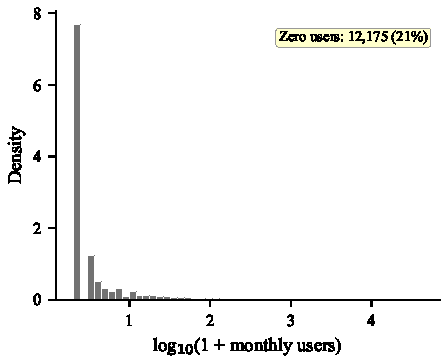
\includegraphics[width=0.7\columnwidth]{figures/F1_usage_distribution}
  \caption{Distribution of monthly users across the 57{,}032 PPE actors (log
    scale). The median actor has one monthly user; the distribution exhibits a
    heavy right tail spanning four orders of magnitude.}
  \label{fig:usage_dist}
\end{figure}

\begin{figure}[t]
  \centering
  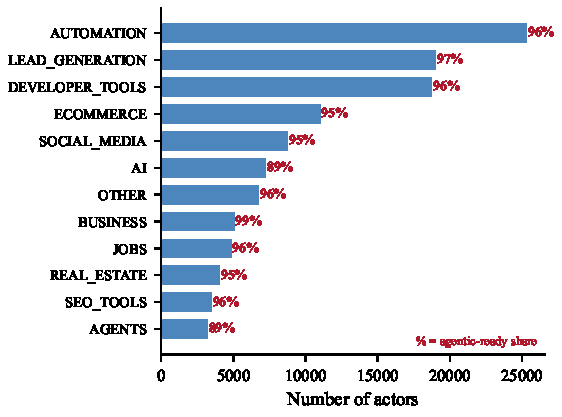
\includegraphics[width=0.7\columnwidth]{figures/F2_category_composition}
  \caption{Category composition of the Apify Store. Bar height shows total
    actor count per category; percentage labels show the agentic-ready share of
    each category.}
  \label{fig:categories}
\end{figure}

%% ─────────────────────────────────────────────
\subsection{Representativeness and Boundary Conditions}

Apify is one of several automation marketplaces (Zapier, UiPath Marketplace,
Bardeen) sharing the structural properties identified in
\autoref{sec:bg:automation}; it is distinctive in providing a public, crawlable
marketplace with tool-level metadata and an explicit agent-accessible boundary.
One boundary condition is that Apify is not an app store: actors are headless
scripts consumed through API calls, not interactive applications, so the
findings apply most directly to headless automation marketplaces.

%% ─────────────────────────────────────────────
\subsection{The Rental Sunset}

A concurrent institutional change provides context: Apify has announced the
deprecation of rental pricing (October 2026),\footnote{Apify, ``Rental Pricing
Model,'' Apify Documentation,
\url{https://docs.apify.com/actors/publishing/monetize/rental}.} at which point
the remaining 5{,}364 rental actors (8\% of the marketplace) are migrated to
pay-per-usage pricing. Developers who instead want the pay-per-event model must
actively migrate their actors themselves. A rental actor that a developer
converts to pay-per-event becomes eligible for agentic readiness only if it is
also configured with limited permissions and no standby; its full effects unfold
after our observation window.

% !TEX root = ../main.tex
\section{Data and Method}
\label{sec:method}

This section describes data collection, variable operationalization, and the
analytic strategies used to address each research question.

%% ----------------------------------------------------------------
\subsection{Data Collection}
\label{sec:data}

Our data come from the Apify Store's public REST API, which exposes actor-level
metadata, usage statistics, pricing structures, and developer information. The
API returns paginated JSON responses that include storefront fields plus
structured metadata such as event-level pricing and category identifiers. We
additionally query the actor-detail endpoint \texttt{GET /v2/acts/\{actorId\}}
to retrieve each tool's \texttt{actorPermissionLevel} and
\texttt{actorStandby}---the two architectural fields that operationalize
agentic readiness (\autoref{sec:variables}).

\paragraph{Enumeration and coverage.}
The global search endpoint truncates results at roughly 15{,}000 actors, so we
enumerate via the public sitemap: we extract 5{,}400+ developer usernames, then
issue per-developer paginated queries. We set \texttt{includeUnrunnableActors=true}
on every query so actors excluded by the API's default runnability filter are
retained. This two-stage strategy covers the full marketplace: every actor
belongs to exactly one developer, and every developer with a public actor
appears in the sitemap.

\paragraph{Snapshots and validation.}
We collected 17 daily snapshots (2026-08-19 to 2026-09-04); all
cross-sectional analyses use the latest (2026-09-04). The actor-detail endpoint
was queried on 2026-08-27, so the two architectural fields that define agentic
readiness (permission level and standby) are measured once. The remaining
snapshots serve for validation: zero duplicate rows, high actor retention, and
stability of the store's agentic-payments whitelist flag (recorded daily from
the store listing; only 1.4\% of actors change state across the 17 days).
Because the whitelist flag is a platform-side summary of agentic eligibility
that incorporates the architectural criteria among its inputs, its stability is
suggestive---but not conclusive---of architectural stability, which we cannot
observe daily. The single-snapshot census is 67{,}609 actors from
5{,}789 developers; among the 57{,}032 pay-per-event (PPE) actors, the detail
endpoint returned permission and standby fields for 53{,}502, of which 50{,}917
(95\%) are agentic-ready.

\paragraph{Ethics.} All data are public and require no authentication; the
dataset contains no personal data beyond public developer usernames.

\paragraph{Analytic samples.} Three nested samples structure the analyses: the
\emph{full marketplace} ($N = 67{,}609$), the \emph{PPE sample}
($N = 57{,}032$; 53{,}502 with architecture fields), and the
\emph{mixed-developer PPE sample} ($N = 343$ developers, 16{,}537 actors) that
publish both agentic-ready and non-agentic-ready tools and support the
within-developer fixed-effects design.

%% ----------------------------------------------------------------
\subsection{Variables and Operationalization}
\label{sec:variables}

\paragraph{Outcome.}
Our primary outcome is $\log(1 + \texttt{monthly\_users})$, the breadth of an
actor's user base over the trailing 30 days. We use the log-plus-one transform
because adoption counts are heavily right-skewed (median 1, top actors in the
tens of thousands); percentages reported as $\exp(\hat\beta) - 1$ refer to the
$1 + \texttt{monthly\_users}$ scale, not monthly users itself. As a secondary
outcome we use $\log(1 + \texttt{runs\_30d})$.

\paragraph{Treatment variable.}
The treatment is \emph{agentic readiness}, a binary indicator equal to one when
a PPE tool is configured with \emph{limited permissions} and \emph{no standby
mode}. We operationalize it from two actor-detail fields:
\texttt{actorPermissionLevel} ($\texttt{LIMITED\_PERMISSIONS}$ vs.\
$\texttt{FULL\_PERMISSIONS}$) and \texttt{actorStandby}/\texttt{standbyUrl}
(standby enabled vs.\ not). A tool is agentic-ready when it is
limited-permissions and non-standby. These two fields are the
\emph{architectural} component of Apify's agentic-payment eligibility
(\autoref{sec:context}): they are necessary conditions that the developer sets
in the tool's architecture, distinct from the developer-level KYC and
approval-level curation gates that the platform applies on top of them. Agentic
readiness thus describes \emph{architectural} admission to the agent-accessible
set---the tools the platform's architecture renders suitable for AI agents to
discover, invoke, and pay for---not the platform's full approval decision and
not realized agent use; we do not observe whether any given agent invokes a
tool.

\paragraph{Control variables.}
The within-developer specifications control for tool age
($\log(1 + \texttt{age\_days})$), description length, and primary-category fixed
effects, in addition to the developer fixed effects. As a robustness check we
also add further listing-time covariates---log per-event price, log build count,
and the number of pricing events. We do not control for ratings or review
counts, which are post-treatment adoption outcomes rather than confounds. The
per-category regressions instead control for $\log(1 + \texttt{total\_builds})$
(developer effort), developer portfolio size, and the number of pricing events,
because within-developer treatment variation is too sparse in most individual
categories to estimate developer fixed effects reliably.

\paragraph{Category membership.}
Actors are multi-labeled: 84.4\% of PPE actors carry two or three categories.
We define an actor's \emph{primary category} as the first entry in its
platform-returned category list and use primary-category indicators for fixed
effects and per-category regressions; as a robustness check we re-estimate the
per-category results under a multi-hot (any-membership) assignment
(\autoref{sec:results:rq3}).

%% ----------------------------------------------------------------
\subsection{Conceptual Framework}
\label{sec:framework}

Agentic readiness can be associated with adoption through two pathways
(\autoref{fig:mechanism}). The first is \emph{agent-mediated}: readiness
determines which tools enter the feasible interaction set for machine agents,
potentially changing routing and discoverability, which changes the probability
of first adoption and, through popularity feedback, downstream concentration.
The second is \emph{developer-mediated}: the architectural choices that make a
tool agentic-ready---limited permissions, no standby---may be correlated with a
tool's task type, maturity, or target audience. A developer may configure its
mass-market tools with limited permissions while reserving full permission for
complex, enterprise workflows, so readiness is associated with adoption even
without any agent-side routing effect. Such tool-level selection cannot be
ruled out without observing agent traffic.

\begin{figure}[t]
  \centering
  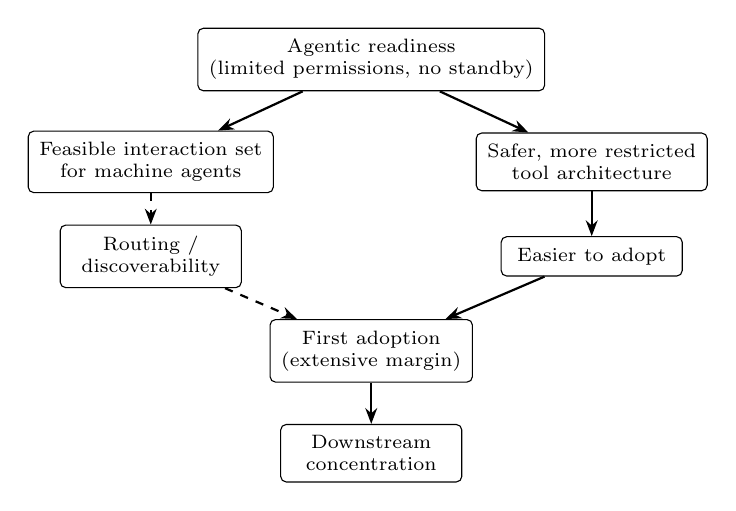
\begin{tikzpicture}[
      box/.style={draw, rounded corners=2pt, align=center, font=\scriptsize, inner sep=4pt, minimum width=2.3cm},
      obs/.style={-{Stealth[length=2mm]}, thick},
      inf/.style={-{Stealth[length=2mm]}, thick, dashed},
    ]
    \node[box] (flag) at (0,0) {Agentic readiness\\(limited permissions, no standby)};
    \node[box] (feasible) at (-2.8,-1.3) {Feasible interaction set\\for machine agents};
    \node[box] (dev) at (2.8,-1.3) {Safer, more restricted\\tool architecture};
    \node[box] (routing) at (-2.8,-2.5) {Routing /\\discoverability};
    \node[box] (choice) at (2.8,-2.5) {Easier to adopt};
    \node[box] (adopt) at (0,-3.7) {First adoption\\(extensive margin)};
    \node[box] (conc) at (0,-5.0) {Downstream\\concentration};
    \draw[obs] (flag) -- (feasible);
    \draw[obs] (flag) -- (dev);
    \draw[inf] (feasible) -- (routing);
    \draw[obs] (dev) -- (choice);
    \draw[inf] (routing) -- (adopt);
    \draw[obs] (choice) -- (adopt);
    \draw[obs] (adopt) -- (conc);
  \end{tikzpicture}
  \caption{Conceptual framework: two pathways from agentic readiness to
    adoption. Solid arrows mark associations we observe; dashed arrows mark
    steps we infer but do not observe. The agent-mediated and developer-mediated
    pathways converge on first adoption and cannot be separated with
    cross-sectional data.}
  \label{fig:mechanism}
\end{figure}

We observe the endpoints of both pathways---agentic readiness and the adoption
outcomes---but not the interior: our data contain no agent-side activity, so the
routing and developer-expectation steps are inferred rather than observed. Our
estimates therefore describe the adoption associated with admission to the
agent-accessible set; attributing this association to agent routing
specifically requires agent-side data. The research questions map onto the
model: RQ1 estimates the total association, RQ2 locates the margin, and RQ3
characterizes concentration.

%% ----------------------------------------------------------------
\subsection{RQ1: Quantifying the Adoption Association of Agentic Readiness}
\label{sec:methods}

We estimate the association between agentic readiness and adoption with a
primary within-developer design and a set of robustness checks.

\subsubsection{Within-Developer Fixed Effects}

The primary specification exploits the 343 developers who publish \emph{both}
agentic-ready and non-agentic-ready pay-per-event tools (16{,}537 actors). For
these mixed developers we estimate
\begin{equation}
\label{eq:fe}
\log(1 + \text{MU}_{ij}) = \beta \cdot \text{Ready}_{ij}
  + \mathbf{X}_{ij} \boldsymbol{\gamma} + \alpha_j + \epsilon_{ij}
\end{equation}
where $\alpha_j$ is a developer fixed effect. The fixed effect absorbs every
time-invariant developer characteristic---reputation, marketing reach, audience
size, category specialization, pricing strategy---so $\beta$ identifies the
\emph{within-developer} contrast between a developer's agentic-ready and
non-agentic-ready tools. This is the strongest comparison our data support: it
holds the developer constant and asks whether readiness predicts adoption
across the tools a single developer publishes. The control vector
$\mathbf{X}_{ij}$ contains tool age, description length, and primary-category
fixed effects; standard errors are clustered at the developer level
\cite{wooldridge2010econometric}.

The design does not address \emph{within-developer selection}: a developer may
configure its most promising tools to be agentic-ready and invest more in them
\cite{boudreau2012complementors}. We treat this as a substantive alternative
explanation rather than a technical nuisance, and return to it in
\autoref{sec:discussion}.

\paragraph{Two estimands.} Developer size correlates with the readiness gap,
so we report two co-equal estimands. The \emph{equal-developer-weighted}
estimand down-weights observations by developer portfolio size: each tool of
developer $j$ receives weight $1/n_j$ (where $n_j$ is the developer's tool
count), so a developer's influence on the estimate does not grow with the number
of tools it publishes. This approximates asking whether the \emph{typical
developer's} agentic-ready tools outperform its non-agentic-ready tools; it
removes the size weighting but not the within-developer variance in readiness
share, so it is not an exact simple average of developer-level contrasts. The
\emph{actor-weighted} estimand weights each tool equally, asking whether the
\emph{typical tool} in the agentic-ready set outperforms the typical tool
outside it. The two answer different questions---one about developers, one about
tools---and we report both throughout (\autoref{sec:results:rq1}).

\paragraph{Who are the mixed developers?} The within-developer design rests on
the 343 mixed developers, a specific subsample rather than a random draw of the
marketplace (\autoref{tab:mixed_developers}). Relative to non-mixed developers,
they run larger portfolios (median 11 versus 2 tools), publish older tools
(median 105 versus 77 days), and attract far more users on average (mean 73.5
versus 11.9 monthly users). They are exclusively boutique-to-whale
developers---no single-tool developer can be mixed by construction. The
within-developer estimates therefore speak to the marketplace's prolific,
established developers rather than to its long tail, a boundary we carry into
the interpretation.

\begin{table}[t]
  \centering
  \caption{The 343 mixed developers versus non-mixed pay-per-event developers.
    Mixed developers publish both agentic-ready and non-agentic-ready tools and
    identify the within-developer effect; non-mixed developers publish only one
    type. Portfolio and age are developer-level; monthly users and agentic-ready
    share are tool-level.}
  \label{tab:mixed_developers}
  \small
  \begin{tabular}{lcc}
    \toprule
    & \textbf{Mixed} & \textbf{Non-mixed} \\
    \midrule
    Developers & 343 & 3{,}826 \\
    Median full-store portfolio & 11 & 2 \\
    Median tool age (days) & 105 & 77 \\
    Mean monthly users & 73.5 & 11.9 \\
    Agentic-ready share (\%) & 91.2 & 97.0 \\
    Solo / Boutique / Mid / Whale (\%) & 0 / 46 / 42 / 12 & 42 / 41 / 15 / 2 \\
    \bottomrule
  \end{tabular}
\end{table}


\subsubsection{Robustness}

Four checks bound the interpretation. First, we exclude \emph{whale developers}
($\geq 100$ pay-per-event tools) and re-estimate the within-developer model, to
rule out that a handful of large developers drive the result. Second, we use
propensity score matching (PSM) \cite{rosenbaum1983propensity, stuart2010matching},
estimating the propensity score from \emph{listing-time} covariates only (tool
age, description length, developer portfolio size, category) so post-treatment
signals cannot enter the model. Because the treated-to-control ratio is 19.7:1,
1:1 matching covers only a small fraction of agentic-ready tools; we therefore
report full-sample weighting estimators---overlap weighting (overlap
population, ATO) and inverse-probability-of-treatment weighting (treated
population, ATT)---alongside 1:1 matching. Because the comparison group is
small and potentially selected, we report covariate-balance diagnostics
(standardized mean differences before and after weighting) and the
propensity-score overlap across the two groups. Third, because
$\log(1+\texttt{monthly\_users})$ compresses the multiplicative gap near zero
(the median tool has one monthly user), we also fit a Poisson
pseudo-maximum-likelihood model with developer fixed effects
\cite{santossilva2006loggravity}, which estimates the gap on the monthly-user
count scale directly. Fourth, to address the
alternative explanation that agentic-ready and non-agentic-ready tools are
simply different tool types, we match each ready tool to its most similar
non-ready tool \emph{within the same developer} (1:1 nearest-neighbor, with
replacement, no caliper) under two similarity notions: description cosine
similarity from TF-IDF vectors (1--2 word n-grams, top 5{,}000 terms), and a
covariate distance (standardized Euclidean distance on log price, log age, and
description length, plus a bonus for an exact category match). For each matched
set we report the mean log-adoption gap with a developer-clustered bootstrap
95\% confidence interval---we resample developers (with replacement) and
recompute the mean gap over the pairs of the sampled developers, since matched
pairs are nested within developers and treating them as independent would
understate uncertainty---and the standardized covariate differences before and
after matching. Because nearest-neighbor matching is a nonsmooth estimator for
which the standard bootstrap is not generally valid
\cite{abadie2006largesample,abadie2008bias}, we treat these intervals as
descriptive rather than as exact inference for the average treatment effect on
the treated.

%% ----------------------------------------------------------------
\subsection{RQ2: Locating the Margin}
\label{sec:methods-rq2}

RQ2 asks \emph{where} the adoption association operates. We decompose it into
an \emph{extensive} margin---whether a tool has any monthly users at all---and
an \emph{intensive} margin---how many users it has conditional on having any.
The distinction maps onto the two pathways in \autoref{fig:mechanism}: an
extensive-margin association is consistent with readiness changing whether a
tool is ever discovered and first adopted, while an intensive-margin
association is consistent with readiness changing how far a tool scales once
adopted. Because the two pathways make different predictions about
\emph{where} the association appears, locating the margin is descriptive.

We estimate three outcomes within the mixed-developer, equal-developer-weighted
design: a linear-probability model for having any monthly users (extensive
margin), an OLS model on $\log(1 + \texttt{monthly\_users})$ conditional on
traction (intensive margin), and a linear-probability model for entering the
top decile of monthly users, which captures the extreme upper tail of adoption.
Each uses developer fixed effects, developer-clustered standard errors, and the
same controls as \autoref{eq:fe}.

%% ----------------------------------------------------------------
\subsection{RQ3: Heterogeneity and Concentration}
\label{sec:methods-rq3}

RQ3 asks two questions: whether the adoption association is uniform across
marketplace categories, and whether agentic readiness is associated with how
concentrated adoption is.

\subsubsection{Category Heterogeneity}

We re-estimate the adoption association separately within each category that
has at least 200 tools and at least 30 in each readiness group (15 categories),
using developer-clustered standard errors and controls for developer effort
($\log(1 + \texttt{total\_builds})$), developer portfolio size, and the number
of pricing events. Because actors are multi-labeled, we report both a
\emph{primary-category} assignment (the first category in the platform-returned
list) and a \emph{multi-hot} (any-membership) assignment, the latter to guard
against tag-ordering artifacts; we apply a Bonferroni correction within each
assignment. Because these per-category regressions use tool-level controls
rather than developer fixed effects, we also estimate a Ready $\times$ Category
interaction in the within-developer model and report within-developer,
within-category estimates where the design supports them, so the category
gradient is not inferred from between-developer variation alone.

\subsubsection{Concentration}

We measure concentration within the agentic-ready and non-agentic-ready sets
separately using three complementary statistics: the Gini coefficient (overall
inequality), top-1\%, top-5\%, and top-10\% user shares (the tail), and a Theil
decomposition into within- and between-category components. We also compare
within-category Gini coefficients across the two sets. The question is whether
admitting agents to a tool set is associated with a more winner-take-all
distribution of users.

% !TEX root = ../main.tex
\section{Results}
\label{sec:results}

Results are organized by research question. Within-developer fixed-effects
models and per-category regressions both cluster standard errors at the
developer level. The full PPE sample has $N = 53{,}502$ actors with architecture
fields (50{,}917 agentic-ready); we report both equal-developer-weighted and
actor-weighted fixed-effects estimates.

%% ─────────────────────────────────────────────
\subsection{RQ1: Agentic Readiness and Adoption}
\label{sec:results:rq1}

Agentic-ready tools are adopted far more than non-agentic-ready tools,
identified among the 343 mixed developers who publish both tool types.
\autoref{tab:eligibility_fe} reports the within-developer fixed-effects
estimates. Within the same developer, agentic-ready tools attract
$\hat\beta = 0.540$ more on the log-plus-one scale (SE $= 0.083$,
$p < 10^{-10}$), i.e., \textbf{71.5\% more on the $(1 + \text{monthly\_users})$
scale} than non-agentic-ready tools under equal-developer weighting. The
actor-weighted estimate is smaller but still large and significant
($\hat\beta = 0.334$, 39.6\%, $p < 10^{-6}$). The divergence between the two estimands indicates the gap is
not uniform across developers: larger portfolios---whose many tools dominate
actor weighting---exhibit smaller within-developer gaps. We treat the
equal-developer-weighted estimate as primary, since it answers the
within-developer question without letting a few large portfolios dominate.

\begin{table}[t]
  \centering
  \caption{Agentic readiness and adoption: within-developer fixed effects.}
  \label{tab:eligibility_fe}
  \small
  \begin{tabular}{lccc}
    \toprule
    Estimator & $\hat\beta$ & exp-1 & 95\% CI \\
    \midrule
    Agentic-ready (equal-developer-weighted) & 0.539 & +71.5\% & [0.38, 0.70] \\
    Agentic-ready (actor-weighted) & 0.334 & +39.6\% & [0.21, 0.46] \\
    \bottomrule
    \multicolumn{4}{l}{\footnotesize Identified among 343 mixed developers (16{,}537 PPE actors), developer-clustered} \\
    \multicolumn{4}{l}{\footnotesize SEs; listing-time controls (age, description, category). Equal-developer-} \\
    \multicolumn{4}{l}{\footnotesize weighted gives each developer equal weight. 95\% CI on the $\hat\beta$ (log) scale.} \\
    \multicolumn{4}{l}{\footnotesize PPML with developer FE (count scale): IRR 8.6, $p=0.012$ (equal-developer-weighted);} \\
    \multicolumn{4}{l}{\footnotesize actor-weighted IRR 2.2, n.s.}
  \end{tabular}
\end{table}

The association is not specific to the monthly-user count. On the secondary
outcome $\log(1 + \texttt{runs\_30d})$---the intensity of tool usage---the
within-developer estimate is $+214\%$ (equal-developer-weighted,
$p < 10^{-17}$) and $+108\%$ (actor-weighted, $p < 10^{-5}$), consistent with
and larger than the breadth result.

The association is robust. Excluding whale developers ($\geq$100 PPE actors) leaves
the equal-developer-weighted estimate essentially unchanged ($\hat\beta = 0.558$,
74.6\%, $p < 10^{-9}$). Adding further listing-time tool-level covariates---log
price, log build count, and the number of pricing events---also leaves the
estimate essentially unchanged (71.5\% to 77.5\%, $p < 10^{-10}$), so the
association is not explained by observable tool-level differences in price or
developer effort. Propensity-score weighting on listing-time covariates
yields estimates of 17\%--24\% depending on the estimator
(\autoref{tab:eligibility_psm}), all positive. These estimates provide directional
triangulation; the
treated-to-control ratio is 19.7:1, and the 2{,}585 non-agentic-ready tools are
systematically older than agentic-ready tools (standardized difference in log
age $-0.90$ before weighting, only partly corrected to $+0.23$ after), with balance diagnostics confirming that the within-developer design remains the better-balanced comparison.

Because ``agentic-ready'' is a conjunction of two architecture choices, the
non-agentic-ready group mixes three configurations. To check whether the gap is
driven by one of them---in particular, by standby mode marking a different,
more enterprise tool type---we decompose the architecture into four cells
(\autoref{tab:architecture_2x2}). Within the same developer, the gap is not
confined to standby: relative to ready (limited, non-standby) tools,
full-permission tools are 50\%--56\% lower in adoption and standby-only tools
24\% lower, so the premium is carried by the permission dimension, with standby
a smaller, secondary contributor.

\begin{table}[t]
  \centering
  \caption{Architecture decomposition: adoption across the four
    permission-by-standby cells. Cells report actor count (mean monthly users).}
  \label{tab:architecture_2x2}
  \small
  \begin{tabular}{lcc}
    \toprule
    & \textbf{Standby} & \textbf{Non-standby} \\
    \midrule
    \textbf{Full permissions} & 57 (4.6) & 1,602 (8.6) \\
    \textbf{Limited permissions} & 926 (10.3) & 50,917 (14.3) \\
    \bottomrule
    \multicolumn{3}{l}{\footnotesize Ready = limited, non-standby (bottom-right). Within-developer, relative to} \\
    \multicolumn{3}{l}{\footnotesize ready: full-permission -50.0\% to -54.9\%; standby-only -24.3\%.}
  \end{tabular}
\end{table}

The association also survives restricting to tools with a full exposure window:
equal-developer-weighted estimates are $+73.0\%$ for tools at least 30 days old,
$+89.2\%$ for tools at least 90 days old, and $+61.6\%$ ($p = 0.002$) for tools
at least 180 days old; replacing $\log(\text{age})$
with age-bin fixed effects leaves the estimate at $+69.5\%$. Across the 343
mixed developers, 65.3\% have a positive within-developer ready--non-ready gap
(median $+0.35$ log points), so the result is not driven by a few developers.

To address the concern that agentic-ready and non-agentic-ready tools are simply
different tool types, we match each ready tool to its most similar non-ready
tool within the same developer (\autoref{sec:methods}). Matching improves
covariate balance (log-age standardized difference $-0.90$ to $-0.30$) and
leaves a positive mean premium of roughly 29\% (developer-clustered bootstrap
95\% CI $[0.06, 0.44]$
log points, versus 72\% unmatched): the adoption premium persists after matching,
though it is attenuated, and the median matched gap is zero with
only 47\% of pairs favoring the ready tool, indicating heterogeneity across
developer--tool pairs.

Because the log-plus-one transform compresses the multiplicative gap near zero
(the median tool has one monthly user), we also fit a Poisson pseudo-maximum-
likelihood model with developer fixed effects, which estimates the gap on the
monthly-user count scale directly. The equal-developer-weighted incidence-rate
ratio is 8.6 ($p = 0.012$), confirming a large count-scale gap among typical
portfolios. The actor-weighted IRR is 2.2 and no longer
statistically significant ($p = 0.268$), reflecting the
disproportionate influence of a few large portfolios whose ready and non-ready
tools are closer in absolute counts. The two magnitudes
describe the same gap at different points of a heavily skewed distribution: the
median tool has one user regardless of readiness, so the log-plus-one estimate
($+40\%$ to $+72\%$) moves the median tool from one to roughly two users. The adoption gap is thus large on the
count scale for most developers, not an artifact of the transform.

\begin{table}[t]
  \centering
  \caption{Propensity-score matching for agentic readiness.}
  \label{tab:eligibility_psm}
  \small
  \begin{tabular}{lcc}
    \toprule
    Estimator & $\hat\beta$ & exp-1 \\
    \midrule
    1:1 nearest-neighbor & 0.192 & +21.2\% \\
    Overlap weighting (ATO) & 0.217 & +24.3\% \\
    IPTW (ATT) & 0.156 & +16.9\% \\
    \bottomrule
    \multicolumn{3}{l}{\footnotesize Listing-time propensity score (age, description length,} \\
    \multicolumn{3}{l}{\footnotesize portfolio size, category). Outcome is log-plus-one monthly users.} \\
    \multicolumn{3}{l}{\footnotesize Treated:control = 19.7:1; 1:1 covers a minority of agentic-ready actors.} \\
    \multicolumn{3}{l}{\footnotesize Balance: standardized log-age difference -0.90 before weighting, +0.23 after.}
  \end{tabular}
\end{table}

%% ─────────────────────────────────────────────
\subsection{RQ2: The Margin of Adoption}
\label{sec:results:rq2}

The association appears on both the extensive and conditional intensive
margins (\autoref{tab:eligibility_margins}). On the extensive margin,
agentic-ready tools are \textbf{16.5 percentage points more likely to have any
monthly users} ($p < 10^{-6}$). Conditional on having users, the intensive-margin
association remains large and significant: agentic-ready tools attract
\textbf{60.2\% more} ($p < 10^{-4}$). Entering the top decile is also more
likely for agentic-ready tools ($+10.1$ pp, $p < 10^{-6}$). The association is
thus visible on both margins, consistent with readiness operating through both
discovery and scaling. This two-part decomposition locates where the association appears;
because readiness
itself predicts crossing the zero threshold, the conditional sample of tools
with any users differs in composition between the two groups, so the
intensive-margin estimate is conditional on that selection. Separating agent-mediated from
developer-mediated pathways requires agent-side data (\autoref{fig:mechanism}).

\begin{table}[t]
  \centering
  \caption{Extensive versus intensive margin for agentic readiness.}
  \label{tab:eligibility_margins}
  \small
  \begin{tabular}{lccc}
    \toprule
    Margin & $\hat\beta$ & SE & $p$ \\
    \midrule
    Extensive (any monthly users) & +16.5 pp & 0.032 & <0.001 \\
    Intensive ($\ln(1+\text{MU})$ given MU $>$ 0) & +0.471 & 0.102 & <0.001 \\
    Top decile (MU $\geq$ 10) & +10.1 pp & 0.019 & <0.001 \\
    \bottomrule
    \multicolumn{4}{l}{\footnotesize Within-developer, equal-developer-weighted, developer-clustered SEs.} \\
    \multicolumn{4}{l}{\footnotesize Extensive and top-decile are linear-probability models (coefficient in} \\
    \multicolumn{4}{l}{\footnotesize percentage points); intensive is log-plus-one (coefficient in log points).}
  \end{tabular}
\end{table}

%% ─────────────────────────────────────────────
\subsection{RQ3: Category Heterogeneity and Adoption Inequality}
\label{sec:results:rq3}

\subsubsection{Category heterogeneity.}

The association is positive across most categories in tool-level regressions
(7 of 15 primary-category and 12 of 18 multi-hot are Bonferroni-significant;
\autoref{tab:eligibility_category}). Under developer fixed effects the Ready $\times$ Category interaction is jointly
significant ($F = 6.74$, $p < 10^{-16}$), confirming category-level heterogeneity.
The gradient reorders relative to the tool-level estimates---Agents and AI lose their tool-level
prominence within developer---so the category variation reflects heterogeneity
rather than support for a specific consumer-type mechanism.

\begin{table}[t]
  \centering
  \caption{Per-category agentic-readiness effect (OLS, tool-level controls).}
  \label{tab:eligibility_category}
  \small
  \begin{tabular}{lrcrc}
    \toprule
    Category & Coef. & (SE) & Sig. & $N$ \\
    \midrule
    News             & $+0.6449$ & (0.095) & ***  & 1,231 \\
    Social Media     & $+0.5503$ & (0.116) & ***  & 5,368 \\
    Travel           & $+0.5383$ & (0.150) & ***  & 1,309 \\
    Videos           & $+0.4696$ & (0.165) & **   & 914 \\
    Automation       & $+0.3810$ & (0.058) & ***  & 5,513 \\
    E-commerce       & $+0.3125$ & (0.095) & ***  & 7,364 \\
    Real Estate      & $+0.3047$ & (0.141) & *    & 2,867 \\
    Other            & $+0.2894$ & (0.096) & ***  & 1,209 \\
    AI               & $+0.2882$ & (0.093) & ***  & 3,900 \\
    SEO              & $+0.2361$ & (0.172) & n.s. & 1,548 \\
    Agents           & $+0.2317$ & (0.122) & n.s. & 610 \\
    Jobs             & $+0.2213$ & (0.189) & n.s. & 3,944 \\
    Lead Generation  & $+0.1498$ & (0.141) & n.s. & 8,239 \\
    Developer Tools  & $+0.1192$ & (0.083) & n.s. & 5,747 \\
    MCP Servers      & $-0.1322$ & (0.075) & n.s. & 372 \\
    \bottomrule
    \multicolumn{5}{l}{\footnotesize $^{***}\,p<0.003$ (Bonferroni); $^{**}\,p<0.01$; $^{*}\,p<0.05$; n.s.\,$p\geq 0.05$.} \\
    \multicolumn{5}{l}{\footnotesize Developer-clustered SEs. Controls: log-builds, portfolio size, pricing events.} \\
    \multicolumn{5}{l}{\footnotesize Multi-hot (any-membership) robustness: 12 of 18 categories Bonferroni-significant, all positive.} \\
    \multicolumn{5}{l}{\footnotesize Within-developer (FE) estimates reorder: Agents $-0.10$ and AI $+0.15$ (n.s.);} \\
    \multicolumn{5}{l}{\footnotesize Developer Tools $+0.81$, Social Media $+0.84$, Automation $+0.71$.}
  \end{tabular}
\end{table}

\subsubsection{Within-group adoption inequality.}

We find no robust evidence that adoption is more concentrated among
agentic-ready tools (\autoref{tab:eligibility_concentration}). The Gini
coefficient (the standard scale-invariant measure) is nearly identical across
the two sets (0.935 versus 0.946), with a bootstrap 95\% CI for the difference
of $[-0.04, 0.04]$, narrow around zero; within-category, agentic-ready tools
have a higher Gini in only 7 of 15 categories. There is no reliable evidence of a top-share difference: the face-value gap
(top-1\% 76.8\% versus 74.3\%) has a bootstrap CI of $[-8.7, 25.8]$ pp, consistent with
both no difference and a large one. The total Theil index is higher among
agentic-ready tools (4.13 versus 3.35), but this reflects the agentic-ready
group's larger size and longer tail, and it is no longer distinguishable once
the agentic-ready group is downsampled to the non-agentic-ready size. We
therefore find no detectable concentration premium in the observed readiness
sets.

\begin{table}[t]
  \centering
  \caption{Concentration: agentic-ready versus non-agentic-ready actors.}
  \label{tab:eligibility_concentration}
  \small
  \begin{tabular}{lcc}
    \toprule
    Metric & Agentic-ready & Non-agentic-ready \\
    \midrule
    Gini coefficient & 0.935 & 0.946 \\
    Top 1\% user share & 76.8\% & 74.3\% \\
    Top 5\% user share & 88.7\% & 88.5\% \\
    Top 10\% user share & 92.5\% & 92.4\% \\
    Theil index (total) & 4.13 & 3.35 \\
    Between-category share & 13.1\% & 13.3\% \\
    \bottomrule
    \multicolumn{3}{l}{\footnotesize Within-category Gini higher for agentic-ready in 7 of 15 categories.} \\
    \multicolumn{3}{l}{\footnotesize Bootstrap 95\% CIs for the ready $-$ non-ready difference: Gini $[-0.04, 0.04]$;} \\
    \multicolumn{3}{l}{\footnotesize top-1\% $[-8.7, 25.8]$ pp; top-5\% $[-5.4, 11.7]$ pp; top-10\% $[-3.5, 7.7]$ pp;} \\
    \multicolumn{3}{l}{\footnotesize Theil $[0.07, 2.13]$ (the Theil gap reflects the larger, longer-tailed ready group).} \\
    \multicolumn{3}{l}{\footnotesize Sample-size-equalized (ready downsampled to 2{,}585): Gini CI $[0.85, 0.97]$,} \\
    \multicolumn{3}{l}{\footnotesize top-1\% $[48.3, 89.3]$ pp, Theil $[2.15, 5.33]$---all contain the non-ready values.}
  \end{tabular}
\end{table}

% !TEX root = ../main.tex
\section{Discussion}
\label{sec:discussion}

We document three findings: agentic-ready tools attract far more adoption
(up to 72\% within the same developer), this association appears on both the
extensive and conditional intensive margins, and we find no robust evidence
that adoption is more concentrated among agentic-ready tools. Together they
describe the adoption and concentration patterns associated with the platform's
readiness boundary for machine consumers.

%% ─────────────────────────────────────────────
\subsection{The Adoption Payoff of Agentic Readiness}
\label{sec:discussion:gap}

Within the same developer, agentic-ready tools attract a large and consistently
positive adoption gap---40\% to 72\% on the log-plus-one scale depending on
weighting (72\% under our preferred equal-developer-weighted estimator), and
several-fold larger on the count scale. This is the paper's central finding:
within a developer, the tools configured for agent-initiated use attract
substantially more adoption
than those that are not. The identification strategy isolates readiness, not realized agent activity.

Two pathways can produce this association, and our cross-sectional data cannot
separate them (\autoref{fig:mechanism}). Under an \emph{agent-mediated}
account, agentic-ready tools enter the feasible set agents can discover and
invoke, and this routing raises their adoption. Under a
\emph{developer-mediated} account, the architectural choices that make a tool
agentic-ready may coincide with developer investment or appeal to human
adopters independent of agents, so readiness is associated with adoption even
without any agent-side effect. Both accounts are consistent with the
extensive-margin finding.

Agentic readiness is the \emph{architectural} component of the platform's
agent-access admission, not a proxy we chose. The platform defines limited
permissions and non-standby as necessary architectural conditions for
agentic-payment eligibility; the \texttt{allowsAgenticUsers} filter and the MCP
\texttt{search-actors} tool surface agent-eligible tools to agent discovery, and
agent invocation of ineligible tools is rejected (\autoref{sec:context}). The
treatment therefore measures architectural admission to the agent-accessible
set---a necessary condition for agent use, distinct from the developer-level KYC
and approval-level curation gates the platform applies on top. What remains open
is the \emph{mechanism}: whether the adoption gap reflects agent routing,
correlated tool-level selection---task type, maturity, target audience---or both.

The estimate nonetheless survives excluding whale developers and
propensity-score weighting, so the association is not a small-developer
artifact. The remaining interpretive boundaries---unobserved agent use,
within-developer selection, the identifying subsample, and the temporal
mismatch---are detailed in \autoref{sec:discussion:limitations}.

%% ─────────────────────────────────────────────
\subsection{Within-Group Adoption Inequality}
\label{sec:discussion:concentration}

The paper's second finding is an asymmetry: agentic readiness is associated
with \emph{which tools get adopted}, but not with a \emph{detectable increase
in concentration}. We find no robust evidence that adoption is more
concentrated among agentic-ready tools: Gini coefficients are nearly identical
(0.935 versus 0.946), within categories agentic-ready tools are more
concentrated in only 7 of 15, and a sample-size-equalized comparison shows the
upper-tail gap (top-1\% 76.8\% versus 74.3\%) is too imprecisely estimated to
be informative. These estimates compare concentration within observed readiness sets; market-level counterfactual effects require a different design.

For platform operators, this asymmetry distinguishes access design (who may be
used) from concentration design (how value is distributed), two levers that are
easy to conflate.

%% ─────────────────────────────────────────────
\subsection{Design Implications: Governing Machine Visibility}
\label{sec:discussion:principles}

Our empirical contribution is a large, robust adoption premium attached to
agent-access admission. The conceptual step from it is a design object: the
admission boundary, in which permission architecture doubles as discovery
architecture. That coupling is partly definitional---the platform's
\texttt{allowsAgenticUsers} filter and MCP \texttt{search-actors} surface
limited-permissions, non-standby tools to machine visibility---so the
HCI questions worth asking concern what the coupling does and how to design for it. Three follow.

\emph{The boundary redistributes opportunity, not just access.} Within the same
developer, tools admitted to the agent-accessible set attract substantially more
adoption (40\% to 72\%), and two-thirds of mixed developers have a positive
ready--non-ready gap. An access rule is therefore a distributional lever: it
changes \emph{which tools get adopted}, not merely which tools are technically
admissible. Operators who treat access design as a screening question miss the
governance question of who gains and loses visibility.

\emph{Developers must design for two legibility surfaces.} A tool now has two
distinct interfaces: a visual storefront for humans and a machine-readable
surface---schema, documentation, deterministic execution---for agents. These
require different affordances, and, as API-usability research shows, each
interface must be designed explicitly for its users \cite{myers2016api}; a
developer optimizing for one audience can render the tool illegible to the
other. Dual-audience
legibility is thus not the same task done twice, but two coupled design problems
with different audiences and different success criteria---the central HCI
challenge the boundary creates.

\emph{Platforms must provide dual-audience observability.} Because
\texttt{monthly\_users} collapses human and agent traffic into one number, a
developer---or a platform---cannot tell whether a tool's adoption is
human-driven, agent-driven, or both. As machine-consumer demand grows, the
platform must expose audience-specific traffic and conversion signals, or
developers cannot make informed decisions about how to design for two audiences
whose distinct needs must be balanced---a multisided-fairness concern
\cite{burke2017multisided}.

%% ─────────────────────────────────────────────
\subsection{Limitations and Boundary Conditions}
\label{sec:discussion:limitations}

Several limitations bound the interpretation of our findings.

\emph{Single platform.} All data come from the Apify Store. Whether the
agentic-readiness adoption gap generalizes to other automation marketplaces
(Zapier, UiPath Marketplace, Bardeen) remains an open question.

\emph{Cross-sectional design and temporal mismatch.} Our core analysis uses a
single snapshot, and the treatment is measured at snapshot time while
\texttt{monthly\_users} is a trailing 30-day measure. The architectural fields
that define readiness are measured once (2026-08-27), so we cannot directly
verify that a tool held its architecture state across the full adoption window;
the store's daily whitelist flag is stable (1.4\% of actors change state), which
is suggestive but does not fully resolve the concern.

\emph{No observed agent use.} Agentic readiness describes admission to the
agent-accessible set, not realized agent use; \texttt{monthly\_users} does not
distinguish human from agent traffic, so the agent-mediated and
developer-mediated pathways cannot be separated (\autoref{sec:discussion:gap}).

\emph{Identifying subsample.} The within-developer design is identified by the
343 mixed developers---larger, older, more successful developers---so the
estimate speaks to the marketplace's established developers rather than its long
tail (\autoref{tab:mixed_developers}).

\emph{Control-group imbalance.} Only 5\% of PPE tools are non-agentic-ready, so
the comparison group is small and potentially selected; this most affects the
concentration comparison, which we address with sample-size equalization
(\autoref{sec:discussion:concentration}).

\emph{Residual within-developer selection.} Listing-time covariates barely
attenuate the within-developer coefficient; unobserved tool-level investment
remains the main alternative explanation.

%% ─────────────────────────────────────────────
\subsection{Future Work}
\label{sec:discussion:future}

Future work should study developers who selectively convert rental actors to
pay-per-event (and thus to potential agentic readiness) around the October 2026
sunset, study developers who selectively configure tools to be agentic-ready,
compare automation marketplaces (Zapier, UiPath, Bardeen), and collect
agent-side usage data to separate the agent-mediated and developer-mediated
pathways. Empirically, whether a developer optimizing for one legibility surface
renders the tool illegible to the other remains to be tested, as does how
platforms should surface and evaluate both surfaces---building on API-usability
evaluation methods \cite{myers2016api}.

% !TEX root = ../main.tex
\section{Conclusion}
\label{sec:conclusion}

Analyzing the Apify Store's 67{,}609 tools, we find that the tools a platform
configures for agent-initiated use attract a large and consistently positive
adoption gap: agentic-ready tools attract substantially more monthly users
within the same developer (40\% to 72\% on the log-plus-one scale), spanning both the extensive and
intensive margins.
This adoption premium is not accompanied by a robust concentration increase
among agentic-ready tools (Gini and sample-equalized comparisons show no
reliable difference). The design question for HCI is
therefore not whether to
admit agents, but what architecture admission should require---and who benefits
from the tools a platform makes agent-ready. The study shows that platform readiness boundaries allocate adoption without detectable concentration gains.
Separating agent routing from developer selection and testing generalization across marketplaces are natural next steps.


\bibliographystyle{ACM-Reference-Format}
\bibliography{references}

\end{document}
